\documentclass{article}

\usepackage {amsmath}
\usepackage {setspace}
\usepackage [pdftex]{graphicx}
\usepackage[sort&compress]{achemso}
\usepackage{lineno}

% For typesetting roman numerals
\makeatletter
\newcommand{\rmnum}[1]{\romannumeral #1}
\newcommand{\Rmnum}[1]{\expandafter\@slowromancap\romannumeral #1@}
\makeatother

% some formatting tags
\oddsidemargin  0.0in
\evensidemargin 0.0in
\textwidth      6.5in

\title{Temperature Effects on Surface Sulfur Dioxide}
\author{Eric S. Shamay \and Geraldine L. Richmond}

\begin{document}


\newcommand{\suldiox}{SO$_2$}
\newcommand{\ang}{\,$\textrm{\AA}$}
\newcommand{\angs}{\ang}
\newcommand{\wat}{H$_2$O}

%\maketitle

%\onehalfspacing
\linenumbers 
\doublespacing


%\begin{abstract}
	%...Abstract goes here...
%\end{abstract}

%\section {Introduction}

One of chemistry's many remaining ``black box'' events is the adsorption of a gas into a water surface. Although gas uptake into aqueous systems occurs often environmentally and industrially, we still know very little about the process and the details of the adsorption reactions. How does gas bind to a water surface, and what steps are involved in adsorption? How does a gas molecule near a water surface affect the water to which it will bind? What is the structure of hydrating waters in the surface region, and how does that hydrated solute molecule behave differently than as a gas? Experiments to address these questions provide valuable information, but can never fully describe these microscopic events and behaviors. The information can be determined computationally, and when coupled to the previous experimental work can provide a much more complete picture of gaseous adsorption to aqueous surfaces.

As a model gas, \suldiox~has been used extensively in research because of its importance in commercial and environmental systems. The molecular structure, high solubility in water, and its abundance make it a pivotal compound in numerous aqueous atmospheric reactions. A complete picture of the \suldiox~adsorption process will aide in understanding gaseous adsorption on the many aqueous surfaces in the environment, as well as in understanding the fundamental nature of gases in water interfacial regions. 

In this study we use ab initio quantum molecular dynamics (MD) techniques to model and simulate the hydrating structure that forms around a surface-bound \suldiox~on water. We simulate a dynamic water surface with an extended hydrogen-bonding network that captures the fluidity of the \suldiox~hydrate structures, and the behaviors on the water surface. Unlike small cluster studies that use DFT calculations on geometry optimized structures to find likely geometries in a static vacuum setting, The quantum MD technique allows us to simulate the process much more realistically, and with greater accuracy than our previous classical MD work could allow.\cite{Shamay2011} This computational study greatly enhances the picture developed in our previous work on \suldiox. In our previous computational study we used classical MD to determine net orientational behavior of \suldiox~binding to a water surface, and of the orientation of the waters in response to the presence of an adsorbing gas. Understanding the net behavior of the molecules in the aqueous interfacial region throughout adsorption was the first step to understanding the specific details of gas binding and surface behavior. 

Quantum MD techniques accurately reproduce the hydration geometry around the bound \suldiox~molecules, and allow us to look at the specific bonding interactions that form within the surface hydrates, and in the extended bonding further into the water. The surfaces in this work were simulated at two temperatures: room temperature at 298K, and the more atmospherically relevant cold 270K. This set of temperatures complements our most recent experimental studies that showed the binding of gaseous \suldiox~to a water surface is greatly enhanced at cold temperatures.\cite{Ota2011} Other experiments by our group developed the picture of \suldiox~adsorption, and showed that \suldiox~surface hydrate complexes form when a water surface is exposed to \suldiox~gas.\cite{Tarbuck2005,Tarbuck2006} Conclusions from the experiments regarding the specific nature of those complexes could only be inferred. 

We believe this to be the first temperature study using quantum MD to look at the binding of a small gas molecule to a water surface. We show how temperature affects the bonding behavior of the surface adsorbed \suldiox~to neighboring waters. A proposed set of steps in a binding mechanism for \suldiox~adsorbing to a water surface is presented. We also look at \suldiox~behavior when already bound by the surface waters. Lastly, our analysis shows some interesting extended bonding behavior of \suldiox~hydrates, and that the hydrating waters and the \suldiox~often form cyclic ring structures through intermolecular bonds.

\section{Computational Methods}

On-the-fly ab initio molecular dynamics simulations were performed with the QUICKSTEP package, which is an implementation of the Gaussian plane wave method using the Kohn-Sham formulation of density functional theory (DFT).\cite{VandeVondele2005} The Kohn-Sham orbitals are expanded using a linear combination of atom-centered Gaussian-type orbital functions. The electronic charge density was described using an auxiliary basis set of plane waves. Energies and forces from on-the-fly simulation sampling of the Born-Oppenheimer surface were calculated for each MD step using the Gaussian DZVP basis set, the exchange-correlation functional of Becke, Lee, Yang, and Parr (BLYP),\cite{LEE1988} and the atomic pseudo-potentials of the Goedecker, Teter, and Hutter type.\cite{Goedecker1996} A simulation timestep of 1 fs was used, with a Nose-Hoover thermostat set at 273K and 300K for the ``cold'' and ``hot'' simulations, respectively. These computational parameters were verified to yield a reasonable description of bulk room temperature water when simulating a neat-water system. 

Initially, 10 equilibrated boxes of side-lengths 10.0\angs, with 36 randomly packed water molecules were used. Five of the boxes were used for each of the cold and hot simulations. A sulfur dioxide molecule was randomly placed onto the surface within 2.5\angs~of a water molecule centrally located above the waters in the z-axis. A copy of the initial system cubes were then expanded along one axis (z-axis) to 25\angs. The system energy was minimized through a geometry optimization. Subsequently, the system was equilibrated for 1 ns in canonical ensemble (NVT) conditions. Periodic boundaries were set on the two short axes to form an infinite slab. The equilibrated systems were then simulated for a further 20 ps in the microcanonical ensemble (NVE), with trajectory snapshots recorded every 1 fs. The initial 1 ns equilibration trajectory was not included in the final analysis. This simulation process resulted in 20,000 time steps of system trajectory for analysis in each of the hot and cold replicas of the system, for a total of 100,000 timesteps at each temperature.
 

\section {Sulfur Dioxide Bonding Coordinations}

To further assess the effect of temperature on \suldiox~behavior we turn to analysis of the bonds formed between \suldiox~and the water surface. The bonding coordinations were determined for the \suldiox~based on the bondlength criteria noted in the introduction. Bonds formed between \suldiox-sulfur and \wat-oxygen are labeled 'S' coordinated, and bonds formed between \suldiox-oxygen and \wat-hydrogen are labeled 'O' coordinated. For each bond an additional letter label is appended to the coordination. For example, an 'SOO' coordinated \suldiox~forms three bonds to waters: two bonds are formed through the \suldiox-oxygens, and one through the \suldiox~sulfur. This naming scheme is taken from the work of Baer et al. where the \suldiox~bonding distribution was determined for a surface molecule at a single temperature simulated under similar conditions.\cite{Baer2010}

Figure \ref{fig:so2-bonding-coordinations} shows the distribution of bonding coordinations throughout the set of simulated trajectories for both the cold and hot temperatures.


\begin{figure}[h!]
	\begin{center}
		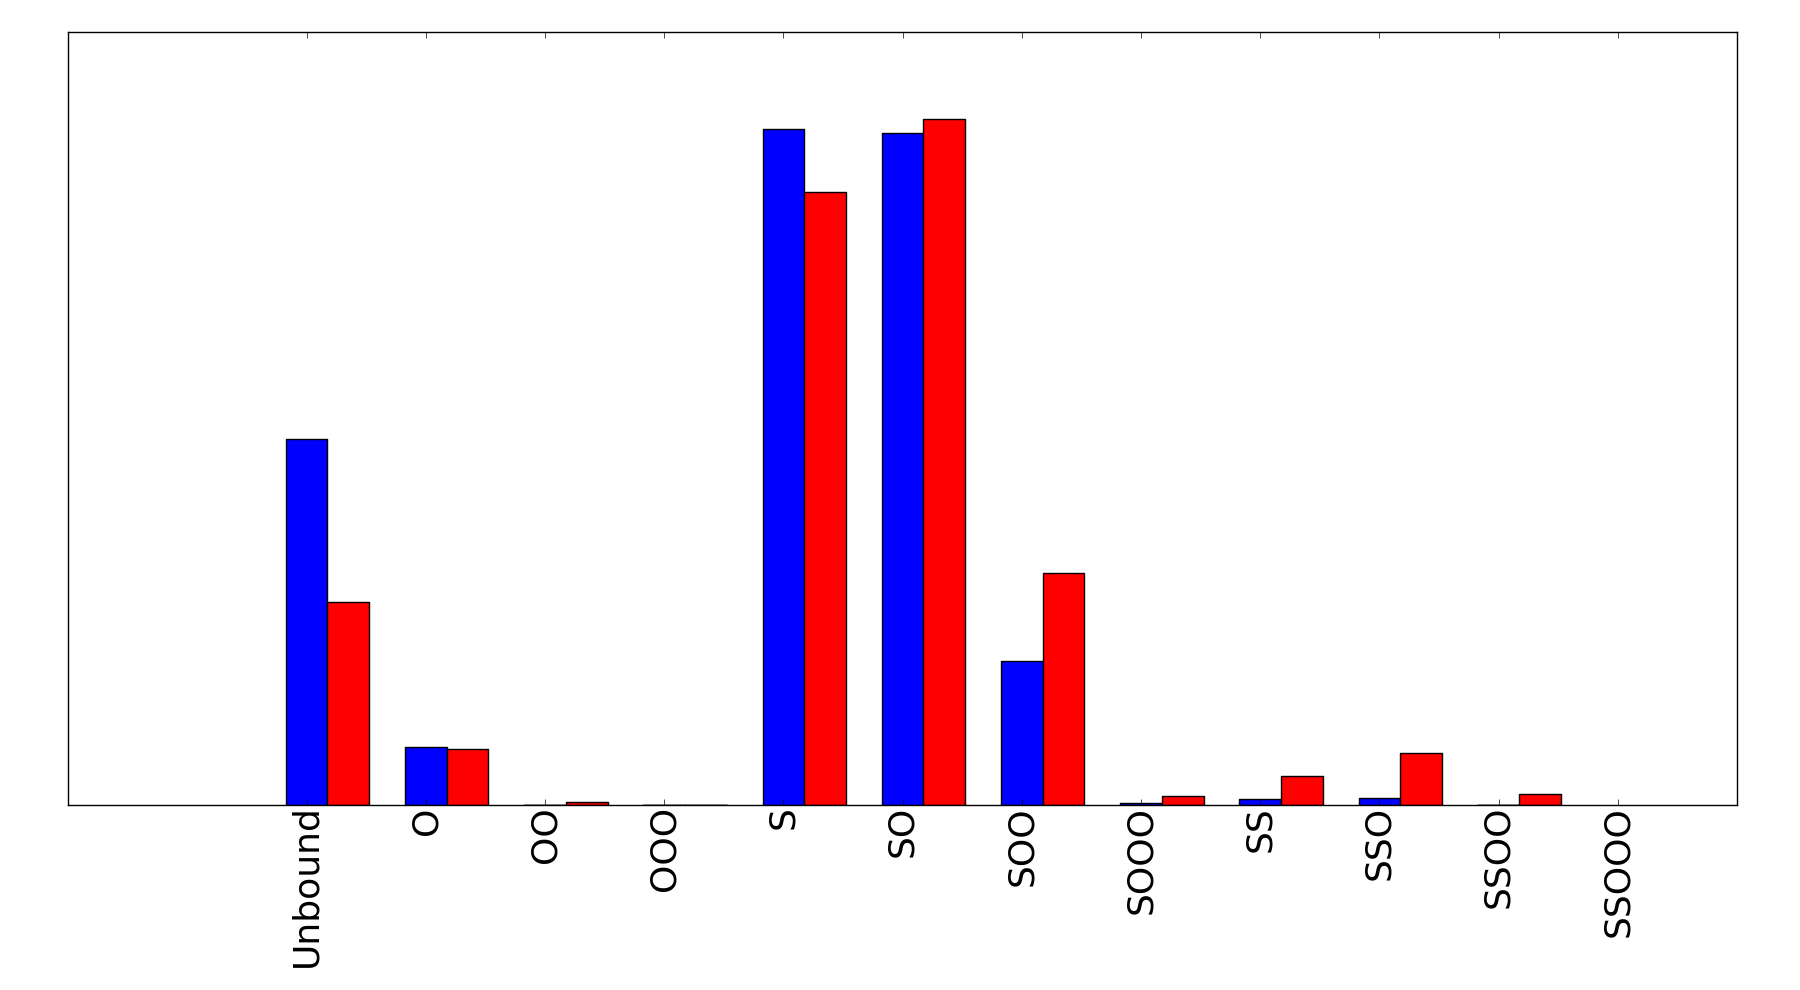
\includegraphics[scale=1.0]{images/coordination/so2-bonding-coordinations.png}
		\caption{}
		\label{fig:so2-bonding-coordinations
	\end{center}
\end{figure}

\section {Liquid Structure}

To further understand the change in \suldiox~surface bonding with changes in temperature we now look at radial distribution functions of the water near the adsorbed \suldiox.

%\include{orientation}
%\include{sfg}
%\include{Results}
%\section {Conclusions}

The adsorption of small gas molecules to water surfaces has been extensively studied over the past few decades. Much has been learned about the energies of hydrate configurations, and the kinetics of gaseous uptake into aqueous systems. Yet, the specific nature of the adsorption process, including the various geometries, hydrate species, and bonding pathways remains largely unknown. As a gas transitions into the liquid water phase, it passes through a fluid interfacial region that remains poorly understood. Our understanding of the processes and chemistry of the interface is still in its infancy, but we gain unique new insights that are key to understanding many environmentally important processes at aqueous surfaces.

Presented herein are the results of ab initio molecular dynamics simulations that focus on how a wandering gaseous \suldiox~molecule first makes contact with a water surface, and subsequently forms extended hydrate structures with interfacial water molecules. The computational studies complement and expand on experimental studies from this laboratory that found surface complexation of \suldiox~at a water surface.\cite{Tarbuck2005,Tarbuck2006,Ota2011} Furthermore, these computations build upon and enrich our understanding of adsorbing \suldiox~behavior from our recently published computational study on interfacial geometries of aqueous surface \suldiox~molecules.\cite{Shamay2011}

Our simulations show that \suldiox~has a preferred means of bonding and interacting with surface water molecules by taking on various bonding coordinations. In this work it was shown that the ``SO'' bonding configuration is the most preferred, with ``S'' and ``SOO'' also contributing greatly to the coordination distribution. Once a \suldiox~has bound to form a surface hydrate it rarely forms multiple bonding interactions through the sulfur atom, and even less frequently takes on a configuration with no sulfur interactions to nearby waters.

This study is one of very few temperature studies looking at the microscopic nature of interfacial gas molecules on water. By changing the temperature, it was found that a hotter water system leads to longer \suldiox~binding to the water surface. The distribution of bonding coordinations was greatly affected by a temperature change, shifting populations of bonding configurations because of the altered \suldiox~and \wat~behavior. At the higher temperature, \suldiox~forms more frequent bonds to interfacial waters through the sulfur and oxygen atoms. Overall, we have determined that the \suldiox~hydrate interactions are transient, binding and unbinding to water molecules rapidly in very dynamic bonding coordinations.

In this work we introduce the use of a graph structure to represent atoms and interconnectedness between molecules, and also to represent transitions between the various bonding coordinations of an adsorbed \suldiox. It was shown that the intermolecular bonds formed through the \suldiox-oxygens are quickly broken and formed, lasting briefly compared to sulfur interactions. From the graph of bonding coordination transitions, we found a likely pathway for \suldiox adsorption starting with an unbound gas-phase \suldiox, ending with a hydrated \suldiox~species bound to surface waters.

The formation of cyclic hydrate structures was probed and it was found that these hydrated bonding ring species form during much of a simulated trajectory. Temperature increases the occurrence of cyclic structures, and also shifts the distribution of the specific types of cycles being formed. Two types of cyclic tri-hydrates were discovered during the course of simulations. The cycle lifetimes were found to be mostly short-lived, with a majority lasting less than 1 ps before breaking and reforming due to the dynamic bonding and motion of the surface waters and \suldiox~molecules. Temperature did not have a very dramatic effect on the cyclic lifespans, but higher temperatures did lead to \suldiox~bonding coordinations that are more likely to form into cyclic hydrates.

These studies build upon our computational and experimental research in this area, seeking to understand how gases adsorb and transit across an aqueous/air interface. Such knowledge is invaluable for understanding land water and environmental aerosol systems where gaseous uptake behavior at a water surface surprises us and often defies our physical intuitions.\cite{Jayne1990,Yang2002,Worsnop1989,Boniface2000}


\bibliography{bib/so2temperature}

\end{document}
